\documentclass[submission,copyright,creativecommons]{eptcs}
% \providecommand{\event}{GraMSec 2014 -- First International Workshop on Graphical Models for Security} % Name of the event you are submitting to
\providecommand{\event}{YR-CONCUR 2017}

% % for printing in early stages, with little margins
\usepackage{times}
% \usepackage[margin=20mm,top=20mm,bottom=20mm]{geometry}
\usepackage[margin=20mm,top=20mm,bottom=40mm]{geometry} %% more bottom space for reviewing

% \documentclass[9pt, english, a4paper]{article}
% \usepackage[latin1]{inputenc}
% \usepackage[T1]{fontenc}
% % \usepackage{babel,graphicx, mathpple, textcomp, varioref, listings, color, colortbl, amssymb, amsthm, amsmath, bbm}
\usepackage{graphicx, mathpple, textcomp, varioref, listings, color, colortbl, amssymb, amsthm, amsmath, bbm}
% \usepackage[affil-it]{authblk}
% \input{kvmacros}
% 
\usepackage[matrix,arrow,cmtip,curve]{xy}
\SelectTips{cm}{}\SilentMatrices\CompileMatrices
% 
\newcommand\cat[1]{\mathfrak{#1}}
\newcommand\Cub{\cat{C}}
\newcommand\Bulk{\cat{B}}
\newcommand\Scul{\cat{S}}
\newcommand\Set{\textup{\textsf{Set}}}
\newcommand\Nat{\mathbbm{N}}
\newtheorem{problem}{Problem}


% \theoremstyle{definition}
% \newtheorem{definition}{Definition}[section]
% \theoremstyle{lemma}
% \newtheorem{lemma}{Lemma}[section]
\newtheorem{theorem}{Theorem}[section]
\newtheorem{lemma}[theorem]{Lemma}
\newtheorem{proposition}[theorem]{Proposition}
\newtheorem{corollary}[theorem]{Corollary}
\newtheorem{property}[theorem]{Property}
\newtheorem{definition}[theorem]{Definition}
\newtheorem{example}{Example}[section]
\newtheorem{exercise}{Exercise}[section]


\begin{document}

\title{Sculptures, ST-structures and Higher Dimensional Automata\thanks{\textbf{Acknowledgements:} I would like to thank my supervisors Christian Johansen and Uli Fahrenberg for their guidance and for including me in a productive conversation about the relation of HDAs and Sculptures resulting in this submission.}}

\author{Christopher A. Trotter %\hspace{1,5cm} Christian Johansen
% \institute{Dept. of Informatics, Univ. of Oslo}
\institute{Dept. of Informatics, University of Oslo, \ -- \ P.O.\ Box 1080 Blindern, N-0316 Oslo, Norway.}
\email{chrisat@ifi.uio.no}
% \and 
% Uli Fahrenberg
% \institute{{\'E}cole Polytechnique, Palaiseau, France}
}
\def\titlerunning{Sculptures, ST-structures and HDAs}
\def\authorrunning{C.A.~Trotter}
% 
% \date{}
% \title{Sculptures, ST-structures and Higher Dimensional Automata}
% 
% \author{Christopher A. Trotter}%
% \affil{Department of Informatics, University of Oslo,\\ P.O. Box 1080 Blindern, N-0316 Oslo, Norway.\\E-mail: chrisat@ifi.uio.no}


\maketitle

\begin{abstract}
	\noindent The main purpose is to provide concrete relationships between highly expressive concurrency models coming from two different schools of thought: the higher dimensional automata, a state-based approach by Pratt and van Glabbeek; and the configuration structures and unrestricted event structures, an event-based approach by van Glabbeek and Plotkin. In this respect, we will define the method of sculpting, described by Pratt, in categorical terms to better understand the event-state duality defined by Pratt. These investigations of sculptures in category theory are intended to provide a better understanding of the relationship between ST-structures, Higher Dimensional Automata and Sculptures in terms of expresiveness. 
	%Moreover, we intend to provide an example of a HDA which can not be sculpted by the categorical definition of a sculpture. 
	%\noindent We will provide a formal description of sculpting which is similar to what Pratt has used in [x] wrt. higher dimensional automata(HDA) and ST-structures(ST). For this task we must deal with the expressiveness and correspondence of the above models. In particular the relationship between the HDAs and sculptures.
\end{abstract}



\section{Introduction}

	In highly concurrency models, Higher Dimensional Automata(HDA) is a state-based approach by Pratt and van Glabbeek and is a geometric model of concurrency that has an attractive aspect which is the automata-like presentation. This aspect is opposed to the event-based model of concurrency, like (prime, flow, (non-)stable) event structures[Pratt MC, Pratt HDA RV, VGlab Exp] or configuration structures such as ST[CJ STs]. Here, I only treat HDAs and ST-structures(ST) which are models of processes that perform actions a, b, c, ... whose internal structure is not further examined. Furthermore, I only study the representation of processes, not representation of operators on processes. I limit myself to models that take a fully asynchronous view on parallelism: whenever a number of actions can happen simultaneously, this must be because they are causally independent, and hence they can also happen in any order.

	%There is an arrow from model A to model B iff there exists a translation from processes representable in model A to processes representable in B that fully respects branching time, causality, and their interplay[VanG, Exp]. Thus, a process and its translation ough to be history preserving bisimulation equivalent[26, 11](in VanG, exp). ST-structures when translated into an HDA have shown to hold up to history preserving bisimulation equivalent($\overset{h}{\sim}$), which has been further investigated in [ST-structures].

	Part of the contribution of this paper is a definition of sculptures in relation to ST-structures and HDAs that may be expressive up to isomorphism. In the latter, we will further discuss these relations.

	%In section 2-3, I introduce the model of higher dimensional automata(HDA) and ST-structures(ST)-, respectively. Then in section 4, I define the notion of sculptures described by Pratt[Pratt, HDA RV]. In section 5, I briefly discuss the embedding of the model of ST-structures into HDA to describe the conflict and duality issue between state-based and event-based concurrency models. Leading to section 6, where I describe future work to be done with sculptures and isomorphic ST and sculptures and embedded HDAs.
	By comparing HDAs through ST, as done in [ST-structures], then we can identify non-isomorphic and non-bisimilar HDAs, as shown by Figure 6 in [ST-structure], such that non-isomorphic HDAs can be collapsed into isomorphic ST. Providing us with an example of the perfect duality paradox described by Pratt[HDA revisited]. It follow that the more interesting figure of figure 6(left) in [ST-structure] is due to subleties that evaporate when considering processes up to isomorphism, and even hereditary history preserving bisimular equivalence. We will compare Sculptures to ST by showing that isomorphism holds and investigate HDAs embedded into Sculptures.

	%If I compare HDAs through ST, then we can identify non-isomorpic and non-bisimilar which one can see by the figure 1 that non-isomorphic HDAs can be collapsed into isomorphic ST. Providing the perfect duality paradox mentioned by Pratt[HDA revisited]. It follows that the more interesting figure of figure 1 is due to causal subleties that evaporate when considering processes up to isomorpism, and even hereditary history preserving bisimular. We will compare Sculptures to ST by showing that isomorphism holds and investigate if HDAs can be embedded into Sculptures.

	%Part of the contribution of this paper is a definition of sculptures in relation to ST-structures and HDAs such

	
	%In highly concurrency models, Higher Dimensional Automata(HDA) is a state-based approach by Pratt and van Glabbeek and is a geometric model of concurrency that has an attractive aspect which is the automata-like presentation. This aspect is opposed to the event-based models of concurrency, like (prime, flow, (non-)stable) event structures[1, 2, 3] or configuration structures such as ST[4]. Here, I only treat HDAs and ST-structures(ST) which are models of processes that perform actions a, b, c, ... whose internal structure is not further examined. Furthermore, I only study the representation of processes, not representation of operators on processes. I restrict myself to models that take branching time fully into account, and hence skip models that represent processes by the set of their executions. Thus, the expressive power of the models differ only to the extent that certain forms of causal dependence are expressible. I limit myself to models that take a fully asynchronous view on parallelism: whenever a number of actions can happen simultaneously, this must be because they are causally independent, and hence they can also happen in any order.

	%There is an arrow from model A to a model B iff there exists a translation from processes representable in model A to processes representable in B that fully respect branching time, causality, and their interplay[VanG, Exp]. Thus, a process and its translation ough to be history preserving bisimulation equivalent[26, 11](in VanG, exp).

	%Part of the contribution of this paper is a definition of sculptures in relation to ST-structures that are expressive up to preserving bisimulation equivalence and HDAs that are expressive up to isomorphism. We will discuss these in relation to eachother.


	%If I compare ST and HDA up to ST-bisimulation equivalence one can see by the figure 1 that the ST describes two HDAs that seem to be different. It follows that the more interesting figure of figure 6 is due to causal subleties that evaporate when considering processes up to ST-bisimulation equivalence. We will comapre both HDA given by the ST-bisimulation equivalence and show a equivalence up to isomorphism.
	
	%Here, I only treat models of processes that perform actions a, b, c, ..., whose internal structure is not further examined and real-time and stochastic aspects of processes are completely ignored. Furthermore, I only study the representation of processes, not representation of operators on processes. I restrict myself to models that take branching time fully into account, and hence skip models that represent processes by the sets of their executions. Thus, the expressive power of the models differ only to the extent that certain forms of causal dependence are expressible. I limit myself to model that take a fully asynchronous view on parallelism: whenever a number of actions can happen simultaneously, this must be because they are causally independent, and hence they can also happen in any order.


	%In highly expressive concurrency models, HDA is a state-based approach by Pratt and van Glabeek and is a geometric model of concurrency that has an attractive aspect which is the automata-like presentation. This aspect is opposed to the event-based models of concurrency, like (prime, flow, (non-)stable) event structures [x, y, z] or configuration structures such as ST.\\

	%One of the most commonly used models of concurrency is that of automata, also known as process graphs, state transition diagrams or labelled transition systems. In ordinary automata, the parallel composition of two actions a and b is displayed as a process P that executes a and b in either order, ending in the same state each way, such that a and b are mutually exclusive. Throughout the years, people have wondered whether the elegance of automata could be combined with the expresiveness of models like (prime, flow, (non-)stable) event structures[5, 6, 7] or configuration structures and unrestricted event structures[8, 9]. The geometric model of concurrency, studied by Pratt and van Glabbeek [1, 2, 3], is of high expressive power, thus providing a general framework for studying the difference and common features of various other models of concurrency(as done in [3] and [4]). This model was named Higher Dimensional Automata(HDA) by Pratt[1]. An attractive aspect of HDA is the automata-like presentation[3], which emphasizes the state aspect of the modelled system(and transitions between states). The idea of HDA had to some extent been contempllated before in [28] and applied in [23]. However, [24] offered the first formalisation of the idea and Pratt's formalisation was based on n-categories.

	%Throughout the years, people have wondered whether the elegance of automata could be combined with the expressiveness of models like (prime, flow, (non-)stable) event structures[5, 6, 7] or configuration structures and unrestricted event structures[8, 9]. 



	%One of the most commonly used models of concurrency is that of automata, also known as process graphs, state transition diagram or labelled transition systems. In ordinary automata, the parallel composition P of two actions a and b is displayed in the same way as a system M that executes a and  b in either order, ending in the same state each way, such that a and b are mutually exclusive.

	%One of the most commonly used models of concurrency is that of automata, also known as process graphs, state transition diagrams or labelled transition systems. In ordinary automata, the parallel composition of two actions \emph{a} and \emph{b} is displayed as a process \emph{P} that executes \emph{a} and \emph{b} in either order, ending in the same state each way, such that \emph{a} and \emph{b} are mutually exclusive. There is a hidden assumption of excluded middle as described by Pratt in \cite{pratt1991}, such that the dual of a true concurrency schedule appears to be a false concurrency automaton.

	%This has lead to the geometric model of concurrency, studied by Pratt and van Glabbeek \cite{pratt1991, pratt2000, glab2006}, which is of high expressive power, thus providing a general framework for studying the difference and common features of various other models of concurrency(as done in \cite{glab2006} and \cite{goub2012}). This model was named Higher Dimensional Automata(HDA) by Pratt\cite{pratt1991}. HDAs retained the state-based view and models $a||b$ as the evident four-state $"$square$"$ automaton accepting ab + ba, but with its square interior filled in(Section 2). This aspect is opposed to the event-based model of concurrency, like (prime, flow, (non-)stable) event structures\cite{winsk1979, winsk1986,castell1989} or configuration structures and unrestricted event structures\cite{glab1995, glab2009}.

	%This lead to
	%In response to the ordinary automata, both event-based and geometry-based approaches to concurrency were developed. Event structures replace the traditional state-based view of computation by the view of $a||b$ as a set $\{a,b\}$ representing two events unconstrained as to order. In contrast the geometry-based approach retains the state-based view and models $a||b$ as the evident four-state $"$square$"$ automaton accepting ab + ba but with its square interior filled in.

	%This lead to the geometric model of concurrency, studied by Pratt and van Glabbeek [1, 2, 3], which is of high expressive power, thus providing a general framework for studying the difference and common features of various other models of concurrency(as done in [3] and [4]). This model was named Higher Dimensional Automata(HDA) by Pratt[1]. An attractive aspect of HDA is the automata-like presentation[3], which emphasizes the state aspect of the modelled system(and transitions between states). This aspect is opposed to the event-based model of concurrency, like (prime, flow, (non-)stable) event structures[5, 6, 7] or configuration structures and unrestricted event structures[8, 9].

	%We are interested in studying such models based on sets of event, but in relation to the state-based model of higher dimensional automata. This study of event-state duality is argued by Pratt\cite{pratt2002}, and the model of chu spaces has been developed in response\cite{gupta1994, pratt1995}.

	%Here the challenge of Pratt with insight from chu spaces and the models based on sets of event, in the spirit of van Glabbeek and Plotkin\cite{glab2009}, are addressed in [ST-paper](Section 3). This model was named ST-structures(ST)[ST-paper]. The relationship between ST-structures and HDAs gives an intuition of the event-state duality described by Pratt, and the method of sculpting gives the relation between ST-structures and HDAs.

	%The geometric model of concurrency, studied by Pratt and van Glabbeek [1, 2, 3], is of high expressive power, thus providing a genereal framework for studying the difference and common features of various other models of concurrency(as done in [3] and [4]). This model was named Higher Dimensional Automata(HDA) by Pratt[1]. An attractive aspect of HDA is the automata-like presentation[3], which emphasizes the state aspect of the modelled system(and transitions between states). This aspect is opposed to the event-based models of concurrency, like (prime, flow, (non-)stable) event structures[5, 6, 7] or configuration structures and unrestricted event structures[8, 9].

	%We are interested in studying such models based on sets of events, but in relation to the state-based model of higher dimensional automata. This study of event-state duality is argued by Pratt[12], and the model of chu spaces has been developed in response[13, 14]. Here the challenge of Pratt, with insight from chu spaces and the developed models based on sets of event, in the spirit of van Glabeek and Plotking[9] have been named ST-structures(ST) in [ST-paper]. The relationship between ST and HDA give an intuition of the event-state duality described by Pratt. In this respect, we provide a formal definition of the method of sculpting which is much like what Pratt has used in [?, 2] to better describe the event-state duality. 


	%The main purpose of this paper is to provide a formal definition of Pratt's notion of sculptures in categorical terms. In this regard, highly expressive concurrency models such as ST-structures(ST) and higher dimensional automata(HDA) have show to have strong relations to the notion of sculptures. In the state-event duality both ST and HDA 

	%- We give a formal method to describe the notion of sculpting based on category theory.
	%- We prove that the HDA example figure can not be sculpted by definition of the formal method.
	%- We provide by the example a counter argument to the notion of sculpting and define a refined notion of sculpting.

	%Note: Start with an example that illustrates the problem. (figure 6 left)

	%1. Describe the problem(the lack of a formal definition of sculpting)\\
	%	- Here is a problem\\
	%	- Its an interesting problem because ...\\
	%	- Its an unsolved problem\\
	%	- here is my claim to solving the problem\\


	%2. State your contribution(A formal method to defining what sculpting is in category theory)\\
	%	- We provide an understanding of the relationships between HDA and ST-structures, ST-structures and sculptures and especially HDA and sculptures.\\
	%	- We give a formal method to describe the notion of sculpting based on category theory.
	%	- We prove that the HDA example figure can not be sculpted by definition of the formal method.
	%	- We provide by the example a counter argument to the notion of sculpting and define a refined notion of sculpting.

	%Note: Start with an example that illustrates the problem. (figure 6 left)

	%Introduce what this concept of sculpting is.
	%Say something about its connection to HDA and ST based on the paper on ST-structures.

	%In highly expressive concurrency models, higher dimensional automata, known as HDA, is a state-based approach by Pratt and van Glabeek. HDA is a geometric model of concurrency that has an attractive aspect which is the automata-like presentation. On the other hand, from a different school of thought there are configuration structures and unrestricted event structures which is a event-based approach by van Glabeek and Plotkin. For the event-based approach, the model of ST-structures which is a configuration structure investigated in [Q] is intended to provide a better understanding of the state-event duality described by Pratt. In this respect we will investigate and formulate the method of sculpting, which is similar to what Pratt has used in [w]. Moreover, we have preliminary results from a categorical approach of the relationship between HDA and sculpting.
	
	%The main purpose is to investigate and formulate sculpting which is similar to what Pratt has used in [z]  wrt. two different school of thought: the higher dimensional automata, a state-based approach by Pratt and van Glabeek; and the configuration structures and unrestricted event structures, an event-based approach by van Glabeek and Plotkin. For the event-based approach, we will investigate ST-structures in [x] to provide a better understanding of the state-event duality described by Pratt. Moreover, we will study the relationships between ST-structures and sculptures, HDA and sculptures and ST-structures and HDA. Especially the relationship between HDA and sculptures based on the notion Pratt provides in [y]. As for providing a more formal description, we have preliminary results from a categorical approach describing the relation of sculptures to HDAs.\\

\section{Higher Dimensional Automata}
	We recall the definition of higher dimensional automata (HDA) following the terminology of [VGlab Exp, VP Trans] and also following additional notions including the restriction to acyclic and non-degenerate HDAS defined in [ST-structure]. A logical study of HDAs can be found in [CJ Modal HDA].

	%We recall the definition of higher dimensional automata (HDA) following the terminology of [VGlab Exp, VP Trans] defining also additional notions including the restriction to acyclic and non-degenerate HDAs. A logical study of HDAs can be found in [CJ Modal HDA].

	For an intuitive understading of the HDA model consider the standard example from [VGlab Exp] pictured in Figure 4. It represents a HDA that models two concurrent events which are labelled by a and b (we can also have the same label a for both events, giving rise to the notion of \emph{autoconcurrency}). The HDA consists of four states $q_{0}^{1}$ to $q_{0}^{4}$, and four transitions between them such that it is the same as the classical picture for the interleaving concurrency, but in the case of HDA there is also a square $q_{2}$. Traversing through the interior of the square means that both events are executing. It is the idea of ''fillilng in the holes'' of traditional automata as described by Pratt in [Pratt HDA Revisited]. When traversing on the lower transition it means that event one is executing but event two has not started yet, whereas, when traversing through the upper transition it means that event one is executing and event two has finished already. In the state $q_{0}^{4}$ both events have finished and in state $q_{0}^{1}$ no event has started yet such that these are the two states where no event is executing.

	%For an intuitive understanding of the HDA model consider the standard example [VGlab Exp, VP Trans] pictured in Figure 4(middle-left). It represents a HDA that models two concurrent events which are labelled by a and b (we can also have the same label a for both events, giving rise to the notion of \emph{autoconcurrency}). The HDA has four states, $q_{0}^{1}$ to $q_{0}^{4}$, and four transitions between them. This would be the classical picture for the interleaving concurrency, but in the case of HDA there is also a square $q_{2}$. Traversing through the interior of the square means that both events are executing. When traversing on the lower transition it means that event one is executiong but event two has not started yet, whereas, whentraversing through the upper transition it means that event one is executing and event two has finished already. In the states there is no event executing; in particular, in state $q_{0}^{4}$ both events have finished, whereas in state $q_{0}^{1}$ no event has started yet.

	Similar, HDAs allow to represent three concurrent events through a cube, or more event through hypercubes. We will follow the terminology of [CJ ST-structures] for HDAs, which is also defined in set theoretical terms in [VGlab Exp].
	

	\begin{definition}{\textbf{(higher dimensional automata [3, Def.1])}}\\
		\indent A cubical set H = (Q, $\bar{s}$, $\bar{t}$) is formed of a family of sets Q=$\cup_{n=0}^{\infty}$ $Q_{n}$ with all sets $Q_{n}$ disjoint, and for each n, a family of maps $s_{i}$, $t_{i}$ : $Q_{n} \rightarrow Q_{n-1}$, with $1 \leq i \leq i \leq n$, which respects the following cubical laws:

		\begin{equation}
		\alpha_{i} \circ \beta_{j} = \beta_{j-1} \circ \alpha_{i},\ 1 \leq i < j \leq n\ and\ \alpha, \beta \in \{s,t\}.
		\end{equation}

		\noindent In H, the $\bar{s}$ and $\bar{t}$ denote the collection of all the maps from all the families (i.e., for all n).A higher dimensional automaton (Q, $\bar{s}$, $\bar{t}$, l, F) over an alphabet $\sigma$ is a cubical set together with a labelling function l:$Q_{1} \rightarrow \sigma$ which respects $l(s_{i}(q))$ = $l(t_{i}(q))$ for all $q \in Q_{2}$ and $i \in \{1,2\}$; and with $I \in Q_{0}$ initial and $F \subset Q_{0}$ final cells.

		The elements of $Q_{0}$ are called nodes and those of $Q_{1}$, $Q_{2}$ and $Q_{3}$ are \emph{edges, square} and \emph{cubes}, respectively. In general, the elements of $Q_{n}$ are called \emph{n-dimensional hypercubes}, or \emph{n-cells}. An n-dimensional hypercube represents a state of a concurrent system in which n transitions are firing concurrently. Because the dimensions of the hypercube are numbered 1,...,n, these transitions are de facto stored as a list.

	\end{definition}



\section{ST-structures}
	We define ST-structures, showing in Section 3 of [CJ ST-structures] that they are a natural extension of configuration structures[VGlab CS:event], and include related notions that stem from the latter. The classical notions of concurrency, causality and conflict are not interdefinable as in the case of event structures or stable configuration structures; but are more loose, as in the case with HDAs.


	\begin{definition}{\textbf{(ST-structures)}}
		An ST-configuration structure(also called ST-structure) is a tuple ST = (E, ST, l) with ST a set of ST-configurations over E satisfying the constraint:
		\begin{equation}
			if(S,\ T) \in ST\ then\ (S,\ S) \in ST,
		\end{equation}
	\noindent and l:$E \rightarrow \sigma$ a labelling function with $\sigma$ the set of labels. We often omit the set of events E from the notation when  there is no danger of confusion.

	The contraint(2) above is a closure, ensuring that we do not represent events that are started but never terminated. The set of all ST-structures is denoted $\mathbb{ST}$. 

	\end{definition}


\section{Sculptures}
	In the cubical set approach to higher dimensional automata an automaton is (possibly infinite) set of cubes of various dimensions. In the Chu space approach one starts instead with a single cube of very large, possibly infinite, dimension and ''sculpts'' the desired process by removing unwanted faces. The axes of the starting cube constitute the events, initially a discrete or unstructured set. The removal of states has the effect of structuring the event set. For example sculpting renders two events equivalent, or synchronized, after all states distinguishing them have been removed.

	The sculpture way of looking at Chu spaces does not reveal the intrinsic symmetry of events and states. An alternative presentation that brings out the symmetry better is as matrix whose rows and columns are indexed by events and states respectively, and whose entries are draw from the set 3=\{0,1,2\}. The column of this matrix constitute the selected faces of the cube.\\

	\noindent(use definition from ST-structure to define Sculptures in terms of HDAs)
	
%prove that HDA is isomorphic to sculptures

%\section{event structures / configuration structures}
\section{Results/just future plans}

\subsection{category theory relate sculptures}
	Let $\Box$ be the small category with objects $\{ 0, 1\}^n$ and morphisms freely generated by $\delta_1^0,\dotsc, \delta_{ n+ 1}^0, \delta_1^1,\dotsc, \delta_{n+1}^1:\{ 0, 1\}^n\to\{ 0, 1\}^{n+1}$ given by

	\begin{equation}
  		\delta_k^\nu( x_1,\dotsc, x_n)=( x_1,\dotsc, x_{ k- 1}, \nu, x_k,\dotsc, x_n)\,,
	\end{equation}
	that is, $\delta_k^\nu$ inserts a $\nu$ into the $k$th position.

	The category of \emph{precubical sets} is $\Cub= \Set^{ \Box^\textup{op}}$, the presheaf category. That is, objects in $\Cub$ are functors $\Box\to \Set$ and morphisms are natural transformations.

	In elementary terms, objects in $\Cub$ are graded sets $X=\{ X_n\}_{n\in \Nat}$ together with face maps $\delta_1^0,\dotsc, \delta_n^0, \delta_1^1,\dotsc, \delta_n^1: X_n\to X_{ n- 1}$ which (automatically) satisfy the precubical identity $\delta_k^\nu \delta_\ell^\mu=\delta_{ \ell-1}^\mu \delta_k^\nu$ for $k< \ell$, and the morphisms are graded functions $f=\{ f_n\}_{ n\in \Nat}$ for which $f \delta=\delta f$.

	By the Yoneda lemma, there is an embedding $\Box^\textup{op}\hookrightarrow \Cub$, the images of which are called \emph{bulks}. Hence a bulk is a precubical set $X$ which is generated by a single (possibly infinite-dimensional) cube.

	Let $\Bulk\subseteq \Cub$ be the induced subcategory of bulks.


	\begin{lemma}
  		Let $f: X\to B$ be a morphism in $\Cub$ with $B\in \Bulk$.  Then $f$ is an embedding.
	\end{lemma}

	\begin{proof}[Sketch]
  		In think this follows directly from the Yoneda lemma, but an elementary proof is not difficult. The essence is that in $B$ there are no loops, hence $f$ cannot send two different cubes to the same image (this would create a loop).
	\end{proof}

	The category $\Scul$ of \emph{sculptures} is the arrow category $\Cub\to \Bulk$. That is, objects in $\Scul$ are $\Cub$-morphisms $X\to B$ with $B\in \Bulk$, and morphisms in $\Scul$ are commutative diagrams
	
	\begin{equation*}
		\xymatrix{X \ar@{^(->}[r] \ar@{^(->}[d] & Y \ar@{^(->}[d] \\ B_1\ar@{^(->}[r] & B_2}
	\end{equation*}
	(Injectivity of $X\to Y$ follows from injectivity of the other three morphisms.)

	There is a (forgetful) functor $U: \Scul\hookrightarrow \Cub$ which ``forgets'' the embeddings into $\Bulk$, i.e.~maps the above diagram to $X\hookrightarrow Y$.

	\begin{problem}
  		Does $U$ have right and/or left adjoints?
	\end{problem}



%\subsubsection{through ST structures}
%\subsection{proof of non-sculpture}
	
	%Model:
	%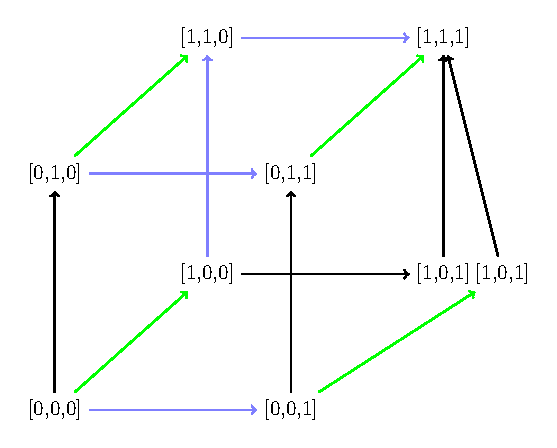
\includegraphics[scale=0.7]{illustrations/figure6.pdf}

	%Pratt gives us the general notion of sculptures, but leaves us without formally defining what this can be. Uli Fahrenberg has given a categorical definition to the high-level abstraction of sculptures and that is given as such.....

	%Having a clear understanding of an abstract notion in itself is a result. This is what should be focused on in the abstraction and be the main motivation for writting the submission to CONCUR. This should be a comparison approach to other formal models... this can be done through comparing Chu Spaces, HDA, ST, Sculptures, etc.

	%We have gotten some preliminary results which are indeed important to determine the concept of a Sculpture and what it means. Also to refine the placement of sculptures meaning that it might be more well behaved than HDAs since there is some information lost in translation between ST and HDA, but ST and Sculptures seem to be equally expressive. So what is the cause of this?

	%NOTE: write out everything that then work on shrinking the ideas and concepts found. This is a good practice to be able to write long and difficult texts as well as getting better at being more concrete and decisive on what is important for the topic.


	%Concurrency theory in theoretical computer science deals with methods, problems and algorithms occurring along with parallel computations. Higher-dimensional Automata are particular models for the study of concurrency; they can be described in a combinatorial/topological manner that takes particular care of the time flow. An analysis of these models has to incorporate direction into tools and methods from algebraic topology and gives rise to \"directed algebraic topology\". The main aim is an analysis of the properties of spaces of executions ( = directed paths) in Higher Dimensional Automata.

% 	\noindent \textbf{Acknowledgement:} I would like to express my special thanks of gratitude to my supervisors Christian Johansen and Uli Fahrenberg for their continuing guidance throughout my master thesis and for including me in a productive conversation about the relation of HDAs and Sculptures resulting in this submission.
	
\bibliographystyle{eptcs}%plain
\bibliography{./references/references.bib}


\end{document}